
%% bare_jrnl_transmag.tex
%% V1.4b
%% 2015/08/26
%% by Michael Shell
%% see http://www.michaelshell.org/
%% for current contact information.
%%
%% This is a skeleton file demonstrating the use of IEEEtran.cls
%% (requires IEEEtran.cls version 1.8b or later) with an IEEE 
%% Transactions on Magnetics journal paper.
%%
%% Support sites:
%% http://www.michaelshell.org/tex/ieeetran/
%% http://www.ctan.org/pkg/ieeetran
%% and
%% http://www.ieee.org/

%%*************************************************************************
%% Legal Notice:
%% This code is offered as-is without any warranty either expressed or
%% implied; without even the implied warranty of MERCHANTABILITY or
%% FITNESS FOR A PARTICULAR PURPOSE! 
%% User assumes all risk.
%% In no event shall the IEEE or any contributor to this code be liable for
%% any damages or losses, including, but not limited to, incidental,
%% consequential, or any other damages, resulting from the use or misuse
%% of any information contained here.
%%
%% All comments are the opinions of their respective authors and are not
%% necessarily endorsed by the IEEE.
%%
%% This work is distributed under the LaTeX Project Public License (LPPL)
%% ( http://www.latex-project.org/ ) version 1.3, and may be freely used,
%% distributed and modified. A copy of the LPPL, version 1.3, is included
%% in the base LaTeX documentation of all distributions of LaTeX released
%% 2003/12/01 or later.
%% Retain all contribution notices and credits.
%% ** Modified files should be clearly indicated as such, including  **
%% ** renaming them and changing author support contact information. **
%%*************************************************************************


% *** Authors should verify (and, if needed, correct) their LaTeX system  ***
% *** with the testflow diagnostic prior to trusting their LaTeX platform ***
% *** with production work. The IEEE's font choices and paper sizes can   ***
% *** trigger bugs that do not appear when using other class files.       ***                          ***
% The testflow support page is at:
% http://www.michaelshell.org/tex/testflow/



\documentclass[journal,transmag]{IEEEtran}
%
% If IEEEtran.cls has not been installed into the LaTeX system files,
% manually specify the path to it like:
% \documentclass[journal]{../sty/IEEEtran}





% Some very useful LaTeX packages include:
% (uncomment the ones you want to load)


% *** MISC UTILITY PACKAGES ***
%
%\usepackage{ifpdf}
% Heiko Oberdiek's ifpdf.sty is very useful if you need conditional
% compilation based on whether the output is pdf or dvi.
% usage:
% \ifpdf
%   % pdf code
% \else
%   % dvi code
% \fi
% The latest version of ifpdf.sty can be obtained from:
% http://www.ctan.org/pkg/ifpdf
% Also, note that IEEEtran.cls V1.7 and later provides a builtin
% \ifCLASSINFOpdf conditional that works the same way.
% When switching from latex to pdflatex and vice-versa, the compiler may
% have to be run twice to clear warning/error messages.






% *** CITATION PACKAGES ***
%
%\usepackage{cite}
% cite.sty was written by Donald Arseneau
% V1.6 and later of IEEEtran pre-defines the format of the cite.sty package
% \cite{} output to follow that of the IEEE. Loading the cite package will
% result in citation numbers being automatically sorted and properly
% "compressed/ranged". e.g., [1], [9], [2], [7], [5], [6] without using
% cite.sty will become [1], [2], [5]--[7], [9] using cite.sty. cite.sty's
% \cite will automatically add leading space, if needed. Use cite.sty's
% noadjust option (cite.sty V3.8 and later) if you want to turn this off
% such as if a citation ever needs to be enclosed in parenthesis.
% cite.sty is already installed on most LaTeX systems. Be sure and use
% version 5.0 (2009-03-20) and later if using hyperref.sty.
% The latest version can be obtained at:
% http://www.ctan.org/pkg/cite
% The documentation is contained in the cite.sty file itself.






% *** GRAPHICS RELATED PACKAGES ***
%
\usepackage{amsmath}
\ifCLASSINFOpdf
   \usepackage[pdftex]{graphicx}
  % declare the path(s) where your graphic files are
   \graphicspath{{../pdf/}{../jpeg/}{../}}
  % and their extensions so you won't have to specify these with
  % every instance of \includegraphics
   \DeclareGraphicsExtensions{.pdf,.jpeg,.png}
\else
  % or other class option (dvipsone, dvipdf, if not using dvips). graphicx
  % will default to the driver specified in the system graphics.cfg if no
  % driver is specified.
   \usepackage[dvips]{graphicx}
  % declare the path(s) where your graphic files are
   \graphicspath{{../eps/}}
  % and their extensions so you won't have to specify these with
  % every instance of \includegraphics
   \DeclareGraphicsExtensions{.eps}
\fi
% graphicx was written by David Carlisle and Sebastian Rahtz. It is
% required if you want graphics, photos, etc. graphicx.sty is already
% installed on most LaTeX systems. The latest version and documentation
% can be obtained at: 
% http://www.ctan.org/pkg/graphicx
% Another good source of documentation is "Using Imported Graphics in
% LaTeX2e" by Keith Reckdahl which can be found at:
% http://www.ctan.org/pkg/epslatex
%
% latex, and pdflatex in dvi mode, support graphics in encapsulated
% postscript (.eps) format. pdflatex in pdf mode supports graphics
% in .pdf, .jpeg, .png and .mps (metapost) formats. Users should ensure
% that all non-photo figures use a vector format (.eps, .pdf, .mps) and
% not a bitmapped formats (.jpeg, .png). The IEEE frowns on bitmapped formats
% which can result in "jaggedy"/blurry rendering of lines and letters as
% well as large increases in file sizes.
%
% You can find documentation about the pdfTeX application at:
% http://www.tug.org/applications/pdftex




% *** MATH PACKAGES ***
%
%\usepackage{amsmath}
% A popular package from the American Mathematical Society that provides
% many useful and powerful commands for dealing with mathematics.
%
% Note that the amsmath package sets \interdisplaylinepenalty to 10000
% thus preventing page breaks from occurring within multiline equations. Use:
%\interdisplaylinepenalty=2500
% after loading amsmath to restore such page breaks as IEEEtran.cls normally
% does. amsmath.sty is already installed on most LaTeX systems. The latest
% version and documentation can be obtained at:
% http://www.ctan.org/pkg/amsmath





% *** SPECIALIZED LIST PACKAGES ***
%
%\usepackage{algorithmic}
% algorithmic.sty was written by Peter Williams and Rogerio Brito.
% This package provides an algorithmic environment fo describing algorithms.
% You can use the algorithmic environment in-text or within a figure
% environment to provide for a floating algorithm. Do NOT use the algorithm
% floating environment provided by algorithm.sty (by the same authors) or
% algorithm2e.sty (by Christophe Fiorio) as the IEEE does not use dedicated
% algorithm float types and packages that provide these will not provide
% correct IEEE style captions. The latest version and documentation of
% algorithmic.sty can be obtained at:
% http://www.ctan.org/pkg/algorithms
% Also of interest may be the (relatively newer and more customizable)
% algorithmicx.sty package by Szasz Janos:
% http://www.ctan.org/pkg/algorithmicx




% *** ALIGNMENT PACKAGES ***
%
%\usepackage{array}
% Frank Mittelbach's and David Carlisle's array.sty patches and improves
% the standard LaTeX2e array and tabular environments to provide better
% appearance and additional user controls. As the default LaTeX2e table
% generation code is lacking to the point of almost being broken with
% respect to the quality of the end results, all users are strongly
% advised to use an enhanced (at the very least that provided by array.sty)
% set of table tools. array.sty is already installed on most systems. The
% latest version and documentation can be obtained at:
% http://www.ctan.org/pkg/array


% IEEEtran contains the IEEEeqnarray family of commands that can be used to
% generate multiline equations as well as matrices, tables, etc., of high
% quality.




% *** SUBFIGURE PACKAGES ***
%\ifCLASSOPTIONcompsoc
%  \usepackage[caption=false,font=normalsize,labelfont=sf,textfont=sf]{subfig}
%\else
%  \usepackage[caption=false,font=footnotesize]{subfig}
%\fi
% subfig.sty, written by Steven Douglas Cochran, is the modern replacement
% for subfigure.sty, the latter of which is no longer maintained and is
% incompatible with some LaTeX packages including fixltx2e. However,
% subfig.sty requires and automatically loads Axel Sommerfeldt's caption.sty
% which will override IEEEtran.cls' handling of captions and this will result
% in non-IEEE style figure/table captions. To prevent this problem, be sure
% and invoke subfig.sty's "caption=false" package option (available since
% subfig.sty version 1.3, 2005/06/28) as this is will preserve IEEEtran.cls
% handling of captions.
% Note that the Computer Society format requires a larger sans serif font
% than the serif footnote size font used in traditional IEEE formatting
% and thus the need to invoke different subfig.sty package options depending
% on whether compsoc mode has been enabled.
%
% The latest version and documentation of subfig.sty can be obtained at:
% http://www.ctan.org/pkg/subfig



% *** FLOAT PACKAGES ***
%
%\usepackage{fixltx2e}
% fixltx2e, the successor to the earlier fix2col.sty, was written by
% Frank Mittelbach and David Carlisle. This package corrects a few problems
% in the LaTeX2e kernel, the most notable of which is that in current
% LaTeX2e releases, the ordering of single and double column floats is not
% guaranteed to be preserved. Thus, an unpatched LaTeX2e can allow a
% single column figure to be placed prior to an earlier double column
% figure.
% Be aware that LaTeX2e kernels dated 2015 and later have fixltx2e.sty's
% corrections already built into the system in which case a warning will
% be issued if an attempt is made to load fixltx2e.sty as it is no longer
% needed.
% The latest version and documentation can be found at:
% http://www.ctan.org/pkg/fixltx2e


%\usepackage{stfloats}
% stfloats.sty was written by Sigitas Tolusis. This package gives LaTeX2e
% the ability to do double column floats at the bottom of the page as well
% as the top. (e.g., "\begin{figure*}[!b]" is not normally possible in
% LaTeX2e). It also provides a command:
%\fnbelowfloat
% to enable the placement of footnotes below bottom floats (the standard
% LaTeX2e kernel puts them above bottom floats). This is an invasive package
% which rewrites many portions of the LaTeX2e float routines. It may not work
% with other packages that modify the LaTeX2e float routines. The latest
% version and documentation can be obtained at:
% http://www.ctan.org/pkg/stfloats
% Do not use the stfloats baselinefloat ability as the IEEE does not allow
% \baselineskip to stretch. Authors submitting work to the IEEE should note
% that the IEEE rarely uses double column equations and that authors should try
% to avoid such use. Do not be tempted to use the cuted.sty or midfloat.sty
% packages (also by Sigitas Tolusis) as the IEEE does not format its papers in
% such ways.
% Do not attempt to use stfloats with fixltx2e as they are incompatible.
% Instead, use Morten Hogholm'a dblfloatfix which combines the features
% of both fixltx2e and stfloats:
%
% \usepackage{dblfloatfix}
% The latest version can be found at:
% http://www.ctan.org/pkg/dblfloatfix




%\ifCLASSOPTIONcaptionsoff
%  \usepackage[nomarkers]{endfloat}
% \let\MYoriglatexcaption\caption
% \renewcommand{\caption}[2][\relax]{\MYoriglatexcaption[#2]{#2}}
%\fi
% endfloat.sty was written by James Darrell McCauley, Jeff Goldberg and 
% Axel Sommerfeldt. This package may be useful when used in conjunction with 
% IEEEtran.cls'  captionsoff option. Some IEEE journals/societies require that
% submissions have lists of figures/tables at the end of the paper and that
% figures/tables without any captions are placed on a page by themselves at
% the end of the document. If needed, the draftcls IEEEtran class option or
% \CLASSINPUTbaselinestretch interface can be used to increase the line
% spacing as well. Be sure and use the nomarkers option of endfloat to
% prevent endfloat from "marking" where the figures would have been placed
% in the text. The two hack lines of code above are a slight modification of
% that suggested by in the endfloat docs (section 8.4.1) to ensure that
% the full captions always appear in the list of figures/tables - even if
% the user used the short optional argument of \caption[]{}.
% IEEE papers do not typically make use of \caption[]'s optional argument,
% so this should not be an issue. A similar trick can be used to disable
% captions of packages such as subfig.sty that lack options to turn off
% the subcaptions:
% For subfig.sty:
% \let\MYorigsubfloat\subfloat
% \renewcommand{\subfloat}[2][\relax]{\MYorigsubfloat[]{#2}}
% However, the above trick will not work if both optional arguments of
% the \subfloat command are used. Furthermore, there needs to be a
% description of each subfigure *somewhere* and endfloat does not add
% subfigure captions to its list of figures. Thus, the best approach is to
% avoid the use of subfigure captions (many IEEE journals avoid them anyway)
% and instead reference/explain all the subfigures within the main caption.
% The latest version of endfloat.sty and its documentation can obtained at:
% http://www.ctan.org/pkg/endfloat
%
% The IEEEtran \ifCLASSOPTIONcaptionsoff conditional can also be used
% later in the document, say, to conditionally put the References on a 
% page by themselves.




% *** PDF, URL AND HYPERLINK PACKAGES ***
%
%\usepackage{url}
% url.sty was written by Donald Arseneau. It provides better support for
% handling and breaking URLs. url.sty is already installed on most LaTeX
% systems. The latest version and documentation can be obtained at:
% http://www.ctan.org/pkg/url
% Basically, \url{my_url_here}.




% *** Do not adjust lengths that control margins, column widths, etc. ***
% *** Do not use packages that alter fonts (such as pslatex).         ***
% There should be no need to do such things with IEEEtran.cls V1.6 and later.
% (Unless specifically asked to do so by the journal or conference you plan
% to submit to, of course. )


% correct bad hyphenation here
\hyphenation{op-tical net-works semi-conduc-tor}


\begin{document}
%
% paper title
% Titles are generally capitalized except for words such as a, an, and, as,
% at, but, by, for, in, nor, of, on, or, the, to and up, which are usually
% not capitalized unless they are the first or last word of the title.
% Linebreaks \\ can be used within to get better formatting as desired.
% Do not put math or special symbols in the title.
\title{Spectrum Sensing for Detection and Radiolocation of UAS}



% author names and affiliations
% transmag papers use the long conference author name format.

\author{\IEEEauthorblockN{Alexander M. Wyglinski\IEEEauthorrefmark{2},
Jonathan M. Peck\IEEEauthorrefmark{1},
Rachel Kinney\IEEEauthorrefmark{1},
Narut Akadejdechapanich\IEEEauthorrefmark{2}, 
Scott Iwanicki\IEEEauthorrefmark{2}, 
Max Li\IEEEauthorrefmark{2}, \\
Kyle Piette\IEEEauthorrefmark{2}, and
Jonas Rogers\IEEEauthorrefmark{2}}
\IEEEauthorblockA{\IEEEauthorrefmark{1}Gryphon Sensors, LLC, North Syracuse, NY 13212}
\IEEEauthorblockA{\IEEEauthorrefmark{2}Worcester Polytechnic Institute, Worcester, MA 01609}% <-this % stops an unwanted space
\thanks{Manuscript received December 1, YYYY; revised August 26, YYYY. 
Corresponding author: J. Peck (email: jpeck@gryphonsensors.com).}}



% The paper headers
\markboth{Journal of \LaTeX\ Class Files,~Vol.~14, No.~8, August~2015}%
{Shell \MakeLowercase{\textit{et al.}}: Bare Demo of IEEEtran.cls for IEEE Transactions on Magnetics Journals}
% The only time the second header will appear is for the odd numbered pages
% after the title page when using the twoside option.
% 
% *** Note that you probably will NOT want to include the author's ***
% *** name in the headers of peer review papers.                   ***
% You can use \ifCLASSOPTIONpeerreview for conditional compilation here if
% you desire.




% If you want to put a publisher's ID mark on the page you can do it like
% this:
%\IEEEpubid{0000--0000/00\$00.00~\copyright~2015 IEEE}
% Remember, if you use this you must call \IEEEpubidadjcol in the second
% column for its text to clear the IEEEpubid mark.



% use for special paper notices
%\IEEEspecialpapernotice{(Invited Paper)}


% for Transactions on Magnetics papers, we must declare the abstract and
% index terms PRIOR to the title within the \IEEEtitleabstractindextext
% IEEEtran command as these need to go into the title area created by
% \maketitle.
% As a general rule, do not put math, special symbols or citations
% in the abstract or keywords.
\IEEEtitleabstractindextext{%
\begin{abstract}
Unmanned Aircraft Systems (UAS), commonly known as drones, are increasingly found in the National Airspace (NAS). However, the use of UAS is not appropriate in all areas or situations. Locating UAS within the airspace is critical for safe integration of UAS into the airspace.  Many sensors that can locate UAS have difficulty differentiating between drones and other small objects in the air, such as birds. This paper presents a ground based spectrum sensor system as a solution to this problem. A spectrum sensor exploits signals emitted by UAS and related equipment for command and control, video, and telemetry data. Detection algorithms are utilized to isolate signals that are emitted by UAS. Following this detection, radiolocation is used to provide the location of the UAS. Similar systems used traditionally in manned aviation are discussed.
\end{abstract}

% Note that keywords are not normally used for peerreview papers.
\begin{IEEEkeywords}
Spectrum Sensing, UAS (Unmanned Aircraft Systems), Radiolocation, ATM (Air Traffic Management), SDR (Software Defined Radio), SAA (Sense and Avoid), DAA (Detect and Avoid), Non-cooperative Sensors.
\end{IEEEkeywords}}



% make the title area
\maketitle


% To allow for easy dual compilation without having to reenter the
% abstract/keywords data, the \IEEEtitleabstractindextext text will
% not be used in maketitle, but will appear (i.e., to be "transported")
% here as \IEEEdisplaynontitleabstractindextext when the compsoc 
% or transmag modes are not selected <OR> if conference mode is selected 
% - because all conference papers position the abstract like regular
% papers do.
\IEEEdisplaynontitleabstractindextext
% \IEEEdisplaynontitleabstractindextext has no effect when using
% compsoc or transmag under a non-conference mode.







% For peer review papers, you can put extra information on the cover
% page as needed:
% \ifCLASSOPTIONpeerreview
% \begin{center} \bfseries EDICS Category: 3-BBND \end{center}
% \fi
%
% For peerreview papers, this IEEEtran command inserts a page break and
% creates the second title. It will be ignored for other modes.
\IEEEpeerreviewmaketitle



\section{Introduction}
% The very first letter is a 2 line initial drop letter followed
% by the rest of the first word in caps.
% 
% form to use if the first word consists of a single letter:
% \IEEEPARstart{A}{demo} file is ....
% 
% form to use if you need the single drop letter followed by
% normal text (unknown if ever used by the IEEE):
% \IEEEPARstart{A}{}demo file is ....
% 
% Some journals put the first two words in caps:
% \IEEEPARstart{T}{his demo} file is ....
% 
% Here we have the typical use of a "T" for an initial drop letter
% and "HIS" in caps to complete the first word.
\IEEEPARstart{T}{he} use of Unmanned Aircraft Systems (UAS), commonly known as drones, is proliferating in the consumer and business markets. The global commercial drone industry is expected to be \$14.9 billon in 2020, with a compound annual growth rate (CAGR) of 8.12\%  year on year [1]. As with traditional aviation, there are safety hazards and privacy concerns with the use of this type of aircraft. To address these concerns and the impending explosion of UAS in the NAS, surveillance of the airspace can monitor the location of objects in the sky, including UAS and manned aircraft. Sensors that provide surveillance data must operate at all hours and in all weather conditions when visibility is reduced. Furthermore, UAS operate at low altitudes where many traditional aviation surveillance sensors cannot detect.

Objects in the airspace are placed into two categories of interest as described in this paper: cooperative and non-cooperative.  Generally, cooperative objects in the airspace are aircraft that are able to determine their own precise geographic location and report it.  Position reporting is traditionally done through a transponder such as ADS-B. However, other wireless technologies have been utilized in UAS for the purpose of position reporting. The term non-cooperatives encompasses a broad set of objects in the sky that aren’t equipped with a transponder.  This includes unequipped manned aircraft, UAS, and birds. This paper only addresses detecting non-cooperatives in the airspace for the safe integration of UAS in the airspace.

Safe integration is used in this paper to describe the safe and harmonious coexistence of manned and unmanned aircraft in the airspace. It is important to note that from a legal standpoint UAS are aircraft. The Federal Aviation Regulation Section 91.113 dictates that an aircraft must be able to “see and avoid” other aircraft.  Current federal regulations such as Part 107 restrict operation of UAS to line-of-sight to the remote pilot. This limits the types of operations that a UAS can undertake. Exceptions to the line-of-sight requirement are granted on a case-by-case basis and must satisfy the “see and avoid” requirement in other ways. This can be accomplished by using sensors for detect and avoid (DAA). 

This paper is organized as follows. First, a literature review of sensors used to detect UAS is provided. The following section defines spectrum sensing, citing recent literature. Elements of a spectrum sensor system are then discussed, along with the heritage of using similar systems in manned aviation. Experimental data is presented that demonstrates the use of a spectrum sensor system to locate a UAS. The paper concludes with a discussion of the limitations of a spectrum sensor system and identifies areas that merit research. 

\section{UAS Detection Methods in Literature}

There are two main categories of sensors used to detect objects in the sky: airborne and ground-based. Airborne sensors are installed on the UAS and are used to sense and avoid other UAS [10]. These types of systems aim to replicate a cockpit view for a pilot or an autopilot system. Ground-based sensors are used to collect surveillance data and are traditionally part of a fixed infrastructure. There are various sensor types discussed in literature for both airborne and ground-based applications. These include LiDAR, optical sensors, thermal infrared sensors, acoustic sensors, and radar.  Brief overviews of different sensors types can be found in [10] and [13]. A more comprehensive discussion of each sensor is provided below.
 
Light detection and ranging (LiDAR) is one technology that has emerged in airborne DAA applications. LiDAR uses a small light or laser shined at the surface of an obstacle and measures the time it takes for the beam to be reflected to its source.  The advantage of LiDAR is that the high level of accuracy enables highly accurate estimations of range and velocity of obstacles. The main drawback of LiDAR is the small volume that it can detect UAS due in part to a narrow field of view. LiDAR systems’ performance is degraded by non-ideal weather conditions, such as rain, fog, mist, snow, and dust. Furthermore, the laser emissions by airborne LiDAR systems may be hazardous to manned aircraft [14]. 
Optical sensor, such as EO/IR cameras, have emerged as a promising technology for UAS detection and collision avoidance both in the air and on the ground. In airborne applications, these sensors provide real-time information on obstructions within the UAS flight path. On a UAS, the performance of these systems is constrained by cost, computational resources, and resolution [10]. Ground-based camera systems have also been proposed for detection of UAS. These systems detect UAS by finding the horizon in order to find objects in the sky [11]. Optical sensors have similar limitations as LIDAR in non-ideal weather conditions. Additionally, their performance is severely degraded in darkness.  The performance of optical sensors are limited by the size of the UAS and the processing available. They have limited performance in tracking multiple targets simultaneously over a wide field of view.

Thermal infrared sensors work much like a camera system. They have a narrow field of view and provide real-time information. Detection requires a UAS to emit heat. Compared to the propulsion systems of manned aircraft, many UAS   radiate far less heat and could be confused with birds. Airborne thermal infrared sensors have also been proposed for obstacle avoidance. In one instance, it has been demonstrated to supply detection data in an indoor environment [15]. The key issues with thermal detection include cost, detection distance, and probability of detection.

Acoustic sensors detect the noise produced by a UAS. Airborne acoustic sensors are effective because they provide intruder detection from all directions [10]. Ground-based acoustic sensors have been demonstrated to be able to detect UAS up to 600 meters and estimate the angle of arrival [12]. In fact, the use of ground based acoustic sensors for the detection of aircraft dates back to before World War I [CITATION NEED]. The limitations of acoustic systems are their limited range and degradation of performance in high noise environments. 

Airborne radar systems have been proposed for DAA on UAS. They can provide an adequate range and field of view for DAA. Airborne radar systems for UAS applications must be small, lightweight, and inexpensive.  Ground-based radars require no additional equipment on the UAS, saving payload for the primary mission. Ground-based radars survey a large volume and can cover multiple UAS. They also serve as a redundant source of position/velocity of craft if communications are lost. Detection of both cooperative and non-cooperative aircraft is possible with either type of radar system. The range of the radar system, both airborne and ground based, is limited by the available power, size of the UAS, and the availability of line-of-sight. 
The merit of radio frequency detection for detection of UAS has been identified [13]. However, radio frequency based detection methods are not well represented in literature. The main contribution of this paper is how to use radio frequency detection methods using a method called spectrum sensing. 

\section{What is Sepectrum Sensing?}
Spectrum sensing is a form of radio frequency detection. It has its roots in cognitive radio. Cognitive radio is generally defined as having the follow functions [6]: 
\begin{itemize}
\item Flexibility and agility to change its operational parameters on the fly such as frequency, waveform, and bandwidth
\item Learning and adaptability to change parameters based on an analysis of the situation
\item Sensing to observe and measure spectrum usage
\end{itemize}
Spectrum sensing is used to provide awareness of the spectrum usage in a given location. In cognitive radio systems, this information is called spectrum opportunities. This term is used due to how this information is traditionally used in a cognitive radio, which is to identify unused spectrum resources that the cognitive radio can use for communication. In addition to cognitive radio, spectrum sensing has been used for other applications. One example is in 802.11 where spectrum sensing is used as part of the medium access control mechanism.

There are various approaches to spectrum sensing. Spectrum sensing can be done independently or collaboratively between sensors. There are various algorithms for spectrum sensing such as energy detection, matched filtering, and cyclostationarity analysis [7]. The aim of these algorithms is to measure the radio frequency energy in one or more domains.  The domains of spectrum usage includes time, frequency, space, angle, and code.

\section{Spectrum Sensing Applied to UAS}
With regard to UAS detection, spectrum sensing is used for identifying spectrum usage by UAS in a specific area.  Spectrum usage is determined by exploiting wireless signals of opportunity emitted by drones. A priori knowledge is utilized to assist in spectrum sensing for UAS in both the frequency and time domain. Once a signal belonging to a UAS is detected through spectrum sensing, the location of the UAS can be estimated through radiolocation techniques.

\subsection{Signals of opportunity emitted by UAS}

Signals of opportunity emitted by UAS are from wireless communications used in UAS. We will only focus on wireless communications used in civil UAS in this discussion.  Currently, there is no single wireless communication protocol that is used in civil UAS. This lack of standardization on a single wireless standard for UAS has led to various wireless technologies being used to satisfy the communication requirement for UAS. Both proprietary and standardized communication protocols are used on UAS.
The type of wireless communication required depends on the UAS use case. Visual line of sight (VLOS) requires the UAS to be within the unaided sight of a remote pilot. Beyond visual line of sight (BVLOS) means that the UAS is flying without the remote pilot having the UAS within visual line of sight at all times. Autonomous UAS are self-guided and do not need to have a remote pilot in control of the craft. The types of wireless communications for each UAS use case is summarized in Table 1 below.

\begin{table}[htbp]
\caption{The Use of Wireless Communication in UAS}
\begin{center}
\begin{tabular}{|c|c|c|c|}
\hline
\textbf{UAS}&\multicolumn{3}{|c|}{\textbf{Wireless Communications}} \\
\cline{2-4} 
\textbf{Use Case} & \textbf{\textit{Command and Control}}& \textbf{\textit{Telemetry}}& \textbf{\textit{Video}} \\
\hline
VLOS& Required& Optional& Optional \\
BVLOS& Required& Required& Optional \\
Autonomous& Required& Optional& Optional \\
\hline
\multicolumn{4}{l}{}
\end{tabular}
\label{tab1}
\end{center}
\end{table}

Command and control is used for a remote pilot to direct a UAS. Command and control communication requires a low bitrate. [9]. As is demonstrated in the literature, there are a variety of frequency bands between 35MHz and 6GHz that are used by command and control data links.  Small UAS typically use traditional remote control radios that often utilize the unlicensed 2.4 GHz band [2]. The emission source for command and control is the ground control station (GCS). 

Telemetry is another low bitrate communication found on a UAS. This information is used to monitor the flight of a UAS. Typical data payloads include the GPS position, IMU measurements, speed, altitude, battery and other status. There are various defined protocols described in [2]. The emission source for telemetry is the UAS.

Live video transmissions is often found on UAS to aid in navigation. Video communication requires a high bitrate radio system. These video transmissions can either be on dedicated hardware or combined with telemetry and command and control hardware. Dedicated video transmitters are often implemented in the 5.8 GHz band. A popular technology used for video links includes 802.11a/b/g/n due to the ease of implementation [2]. The emission source for video is the UAS.

Some wireless technologies can serve multiple communication needs on a UAS. For example, 802.11 meets the bitrate requirements for command and control, telemetry, and video combined. Cellular technology such UMTS and LTE have been demonstrated to do this as well. With these wireless technologies the source of the wireless transmissions isn’t always clear. However, separation of emissions from the UAS and GCS is possible due to the multiplexing of the signals.

\subsection{Spectrum Sensing Algorithms for UAS}

\begin{figure}[htbp]
\centering{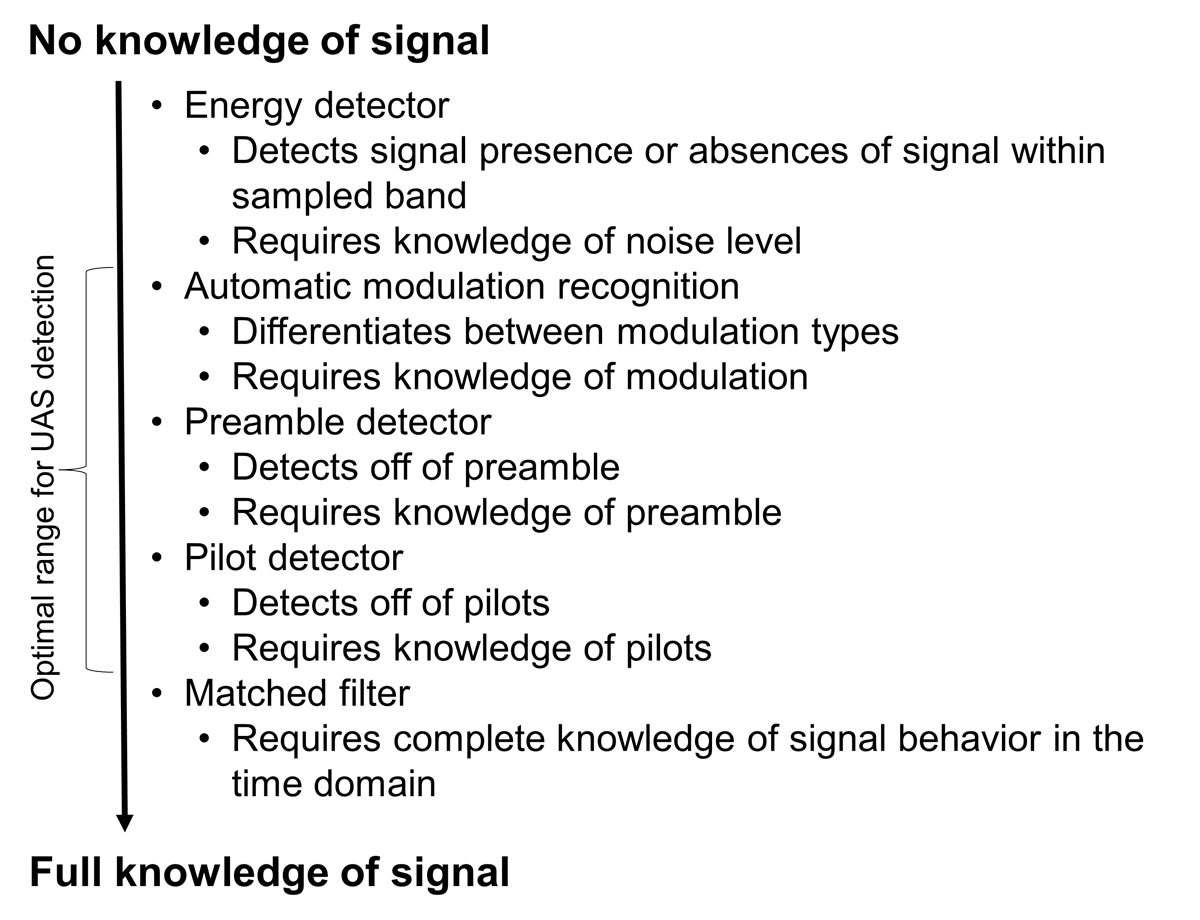
\includegraphics[width=0.4\textwidth]{fig1.png}}
\caption{Spectrum Sensing Algorithms.}
\label{fig}
\end{figure}

As shown in Figure 1, there are various domains in which spectrum sensing can be applied. For UAS, spectrum sensing detection methods are best implemented in either the time domain or frequency domain. This is due to the high level of a priori knowledge that can be collected on UAS wireless links. This information can be gathered from off-the-shelf test equipment, such as a spectrum analyzer.
The spectrum sensing detection algorithms should be implemented in whichever domain there exists a greater understanding of the signal.  For example, if the spectral shape of the signal is well known, but it is unknown if there is any periodic time domain data, such as training data, then a correlation detector (matched filter) implemented in the frequency domain is the optimal detector.  On the other hand, if the spectral characteristics are more random, but signal contains periodic data, such as training data, then time domain detection methods are better.

In some cases, more than one detection method may be appropriate for a signal. Detection methods in one domain may be dependent of knowledge that can be gained by a detector in the other domain. In many cases, time domain detectors require knowledge of the carrier frequency of the signal. This knowledge can be gained using a frequency domain detection method.

Energy detection, a spectrum sensing method commonly used by cognitive radios, is most appropriate if there is little or no knowledge of the signal transmitted. A matched filter (correlator) is the optimal detection method if the spectrum sensor has complete knowledge of signal transmitted. Some spectrum sensing algorithms, such as matched filtering, provide processing gain that increases detection range. Through proper analysis and characterization, the amount of knowledge of transmitted waveforms is somewhere in between the extremes.

Unlike other sensor systems described therein the size of the UAS has no impact on the detection range. The limiting factor of a spectrum sensor is the transmit power of the UAS, processing gain of the detection algorithm, and the antenna gain on the sensor. 

\subsection{Radiolocation}
Radiolocation is the process of determining position of an RF emitter. Throughout aviation history, several approaches to radiolocation have been applied to collision avoidance. One example is the use of a multilateration system to provide aircraft position and identity over the entire Dallas/Ft. Worth airport [3]. A more recent example is a secondary surveillance technique using direction finding in [4]. These are just two examples. More of the history of the use of radiolocation in aviation can be found in [5]. These systems were developed to fill in gaps in surveillance data which were often found through tragic accidents.

Each of these systems, which have been used with larger aircraft, operate on a single wireless transmission standard. These radiolocation systems operate on the basis of having nearly complete knowledge of the signal. As previously mentioned, there are a variety of wireless communication standards used in UAS. Thus, there is less a priori knowledge of the signal compared to systems used in manned aviation. Signal detection and classification using spectrum sensing algorithms provide the majority of the knowledge for radiolocation of UAS.

Traditional radiolocation systems in aviation have a dedicated frequency band. Theses allocated frequency bands are free of interference from other non-aviation related spectrum users. Most civil UAS operate on unlicensed frequency bands. This spectrum is shared with other non-aviation related communication. These systems can interfere with traditional radiolocation methods. It is important to be able to separate UAS RF emissions from non-UAS RF emissions.

Traditional aviation radiolocation systems have cooperative signals. The systems have some control over when signals are emitted and which aircraft emits signals. In contrast, UAS signals are not cooperative with radiolocation systems. Radiolocation systems for UAS must be able to handle collision of signals.

\subsection{Spectrum Sensor System Architecture}

\begin{figure}[htbp]
\centering{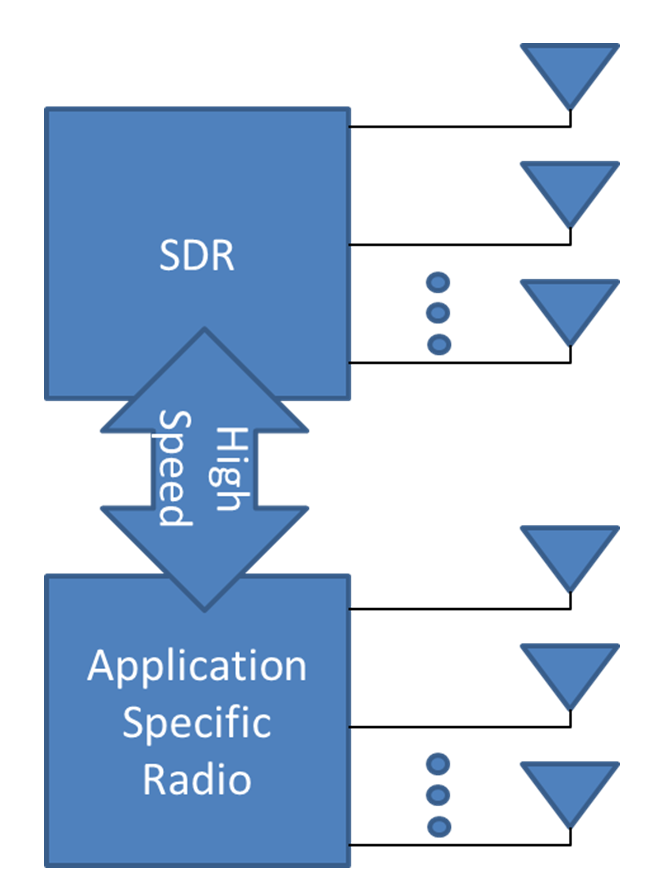
\includegraphics[width=0.4\textwidth]{fig2.png}}
\caption{A high level block diagram of a spectrum sensor.}
\label{fig}
\end{figure}

A sensor node that performs spectrum sensing techniques is called a spectrum sensor. A block diagram of a spectrum sensor is show in Figure 2 above.  A spectrum sensor consists of one or more software defined radios. A software defined radio is a transceiver which signal processing functionalities are performed in a programmable processor. The type of processor can be a digital signal processor, field programmable gate array (FPGA), and/or a general purpose processor [6]. The programmable nature of these radios allows for the spectrum sensor to adapt to new waveforms and frequency bands used by UAS. Coverage of multiple frequency bands is required in order to detect multiple UAS types.

Additional radio receivers for specific wireless standards can optionally be used by the spectrum sensor as well. There exists several wireless chips that implement many of the protocols used by UAS. Examples include RC, 802.11, etc. 

Both the software defined and application specific radios are connected to an antenna system. Depending upon the application, directional or omnidirectional antenna systems can be utilized. The tilt of the directional antennas should be upward to maximize coverage area [8]. 

\section{Limitations of Spectrum Senors}

Spectrum sensing has the best performance when there is a high level of knowledge of the signal of opportunity that is emitted by the UAS. When many of the parameters of a signal are unknown, detection and classification of a UAS are more difficult. Under this condition, performance of a spectrum sensor is limited due to the type of detector that can be applied. Thus, detection performance will be degraded in this case.

The only non-cooperative objects in the airspace that a spectrum sensor works with are ones that emit RF signals on a regular basis. Other non-cooperative objects in the sky, such as birds, balloons, and some general aviation aircraft, do not fall into this category. This limits the usefulness of a spectrum sensor for collision avoidance and safe integration of UAS.

Autonomous UAS may not have any wireless communication signals emitting. These types of UAS may be guided by GNSS or vision alone. UAS that are operated in this manner do not require any periodic communications with the ground. With the absences of any RF signals of opportunity, these UAS cannot be detected by a spectrum sensor. 

A system of systems approach can aid in these scenarios. In a systems of systems approach a spectrum sensor systems can be paired with one or more other types sensors that can detect objects that do not emit RF signals of opportunity. For example, a radar system could be used to complement a spectrum sensor since is capable of detecting objects that do not emit RF signals.


% An example of a floating figure using the graphicx package.
% Note that \label must occur AFTER (or within) \caption.
% For figures, \caption should occur after the \includegraphics.
% Note that IEEEtran v1.7 and later has special internal code that
% is designed to preserve the operation of \label within \caption
% even when the captionsoff option is in effect. However, because
% of issues like this, it may be the safest practice to put all your
% \label just after \caption rather than within \caption{}.
%
% Reminder: the "draftcls" or "draftclsnofoot", not "draft", class
% option should be used if it is desired that the figures are to be
% displayed while in draft mode.
%
%\begin{figure}[!t]
%\centering
%\includegraphics[width=2.5in]{myfigure}
% where an .eps filename suffix will be assumed under latex, 
% and a .pdf suffix will be assumed for pdflatex; or what has been declared
% via \DeclareGraphicsExtensions.
%\caption{Simulation results for the network.}
%\label{fig_sim}
%\end{figure}

% Note that the IEEE typically puts floats only at the top, even when this
% results in a large percentage of a column being occupied by floats.


% An example of a double column floating figure using two subfigures.
% (The subfig.sty package must be loaded for this to work.)
% The subfigure \label commands are set within each subfloat command,
% and the \label for the overall figure must come after \caption.
% \hfil is used as a separator to get equal spacing.
% Watch out that the combined width of all the subfigures on a 
% line do not exceed the text width or a line break will occur.
%
%\begin{figure*}[!t]
%\centering
%\subfloat[Case I]{\includegraphics[width=2.5in]{box}%
%\label{fig_first_case}}
%\hfil
%\subfloat[Case II]{\includegraphics[width=2.5in]{box}%
%\label{fig_second_case}}
%\caption{Simulation results for the network.}
%\label{fig_sim}
%\end{figure*}
%
% Note that often IEEE papers with subfigures do not employ subfigure
% captions (using the optional argument to \subfloat[]), but instead will
% reference/describe all of them (a), (b), etc., within the main caption.
% Be aware that for subfig.sty to generate the (a), (b), etc., subfigure
% labels, the optional argument to \subfloat must be present. If a
% subcaption is not desired, just leave its contents blank,
% e.g., \subfloat[].


% An example of a floating table. Note that, for IEEE style tables, the
% \caption command should come BEFORE the table and, given that table
% captions serve much like titles, are usually capitalized except for words
% such as a, an, and, as, at, but, by, for, in, nor, of, on, or, the, to
% and up, which are usually not capitalized unless they are the first or
% last word of the caption. Table text will default to \footnotesize as
% the IEEE normally uses this smaller font for tables.
% The \label must come after \caption as always.
%
%\begin{table}[!t]
%% increase table row spacing, adjust to taste
%\renewcommand{\arraystretch}{1.3}
% if using array.sty, it might be a good idea to tweak the value of
% \extrarowheight as needed to properly center the text within the cells
%\caption{An Example of a Table}
%\label{table_example}
%\centering
%% Some packages, such as MDW tools, offer better commands for making tables
%% than the plain LaTeX2e tabular which is used here.
%\begin{tabular}{|c||c|}
%\hline
%One & Two\\
%\hline
%Three & Four\\
%\hline
%\end{tabular}
%\end{table}


% Note that the IEEE does not put floats in the very first column
% - or typically anywhere on the first page for that matter. Also,
% in-text middle ("here") positioning is typically not used, but it
% is allowed and encouraged for Computer Society conferences (but
% not Computer Society journals). Most IEEE journals/conferences use
% top floats exclusively. 
% Note that, LaTeX2e, unlike IEEE journals/conferences, places
% footnotes above bottom floats. This can be corrected via the
% \fnbelowfloat command of the stfloats package.

\section{Experimental Results: MAX STUFF HERE, LOOK THROUGH AND REMOVE BAD STUFF}
\subsection{System Integration}
This section details the physical system and the integration of the hardware. This includes power consumption, system layout, and component failures or difficulties. The system diagram shown in Figure \ref{fig:masdr_system_diagram} will be explained in detail in this section.
\begin{figure}[ht!]
  \centering
  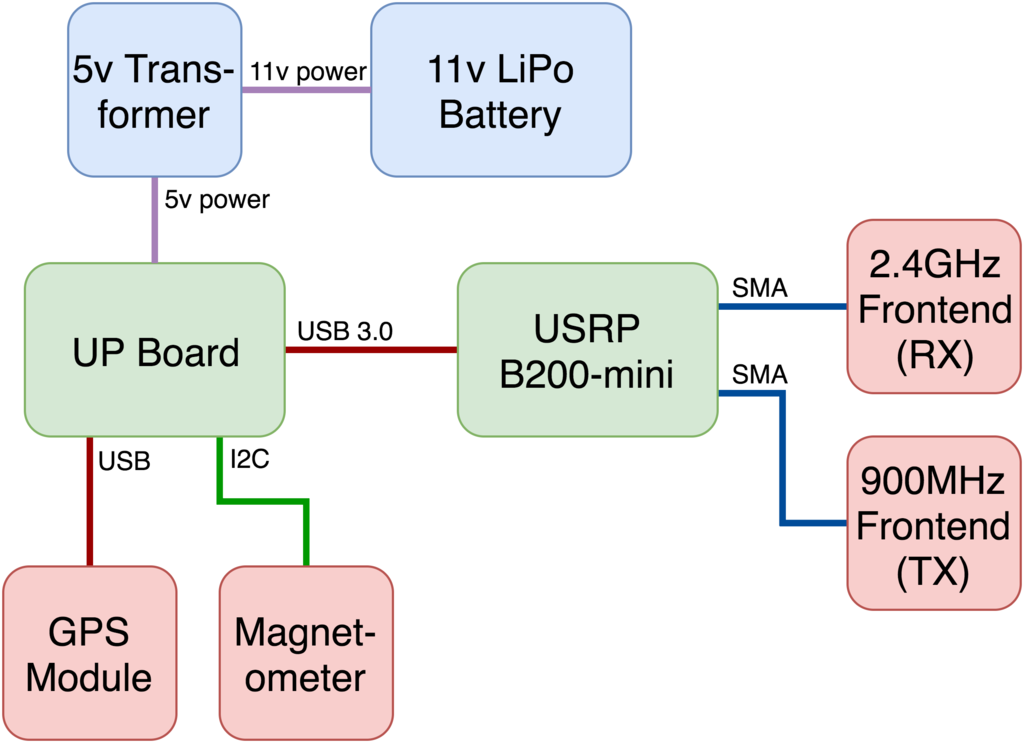
\includegraphics[width=0.45\textwidth]{img/masdr_system_diagram.png}
  \caption{MASDR system diagram detailing the connections between each component.}
  \label{fig:masdr_system_diagram}
\end{figure}\par
\par To power the system, an 11V LiPo battery was used in combination with a 5V transformer to step down the voltage for use by the UP Board. The battery and converter were connected using connectors seen in Figure \ref{fig:connectors}, so that the battery could be disconnected when not in use. To prevent any mishandling of plugging the battery in backwards, a male molex connector was soldered to the transformer and a female molex connector was soldered to the battery.
\par The complete system mounted on the drone is shown in Figure \ref{fig:drone_and_box}.
\begin{figure}[ht!]
  \centering
  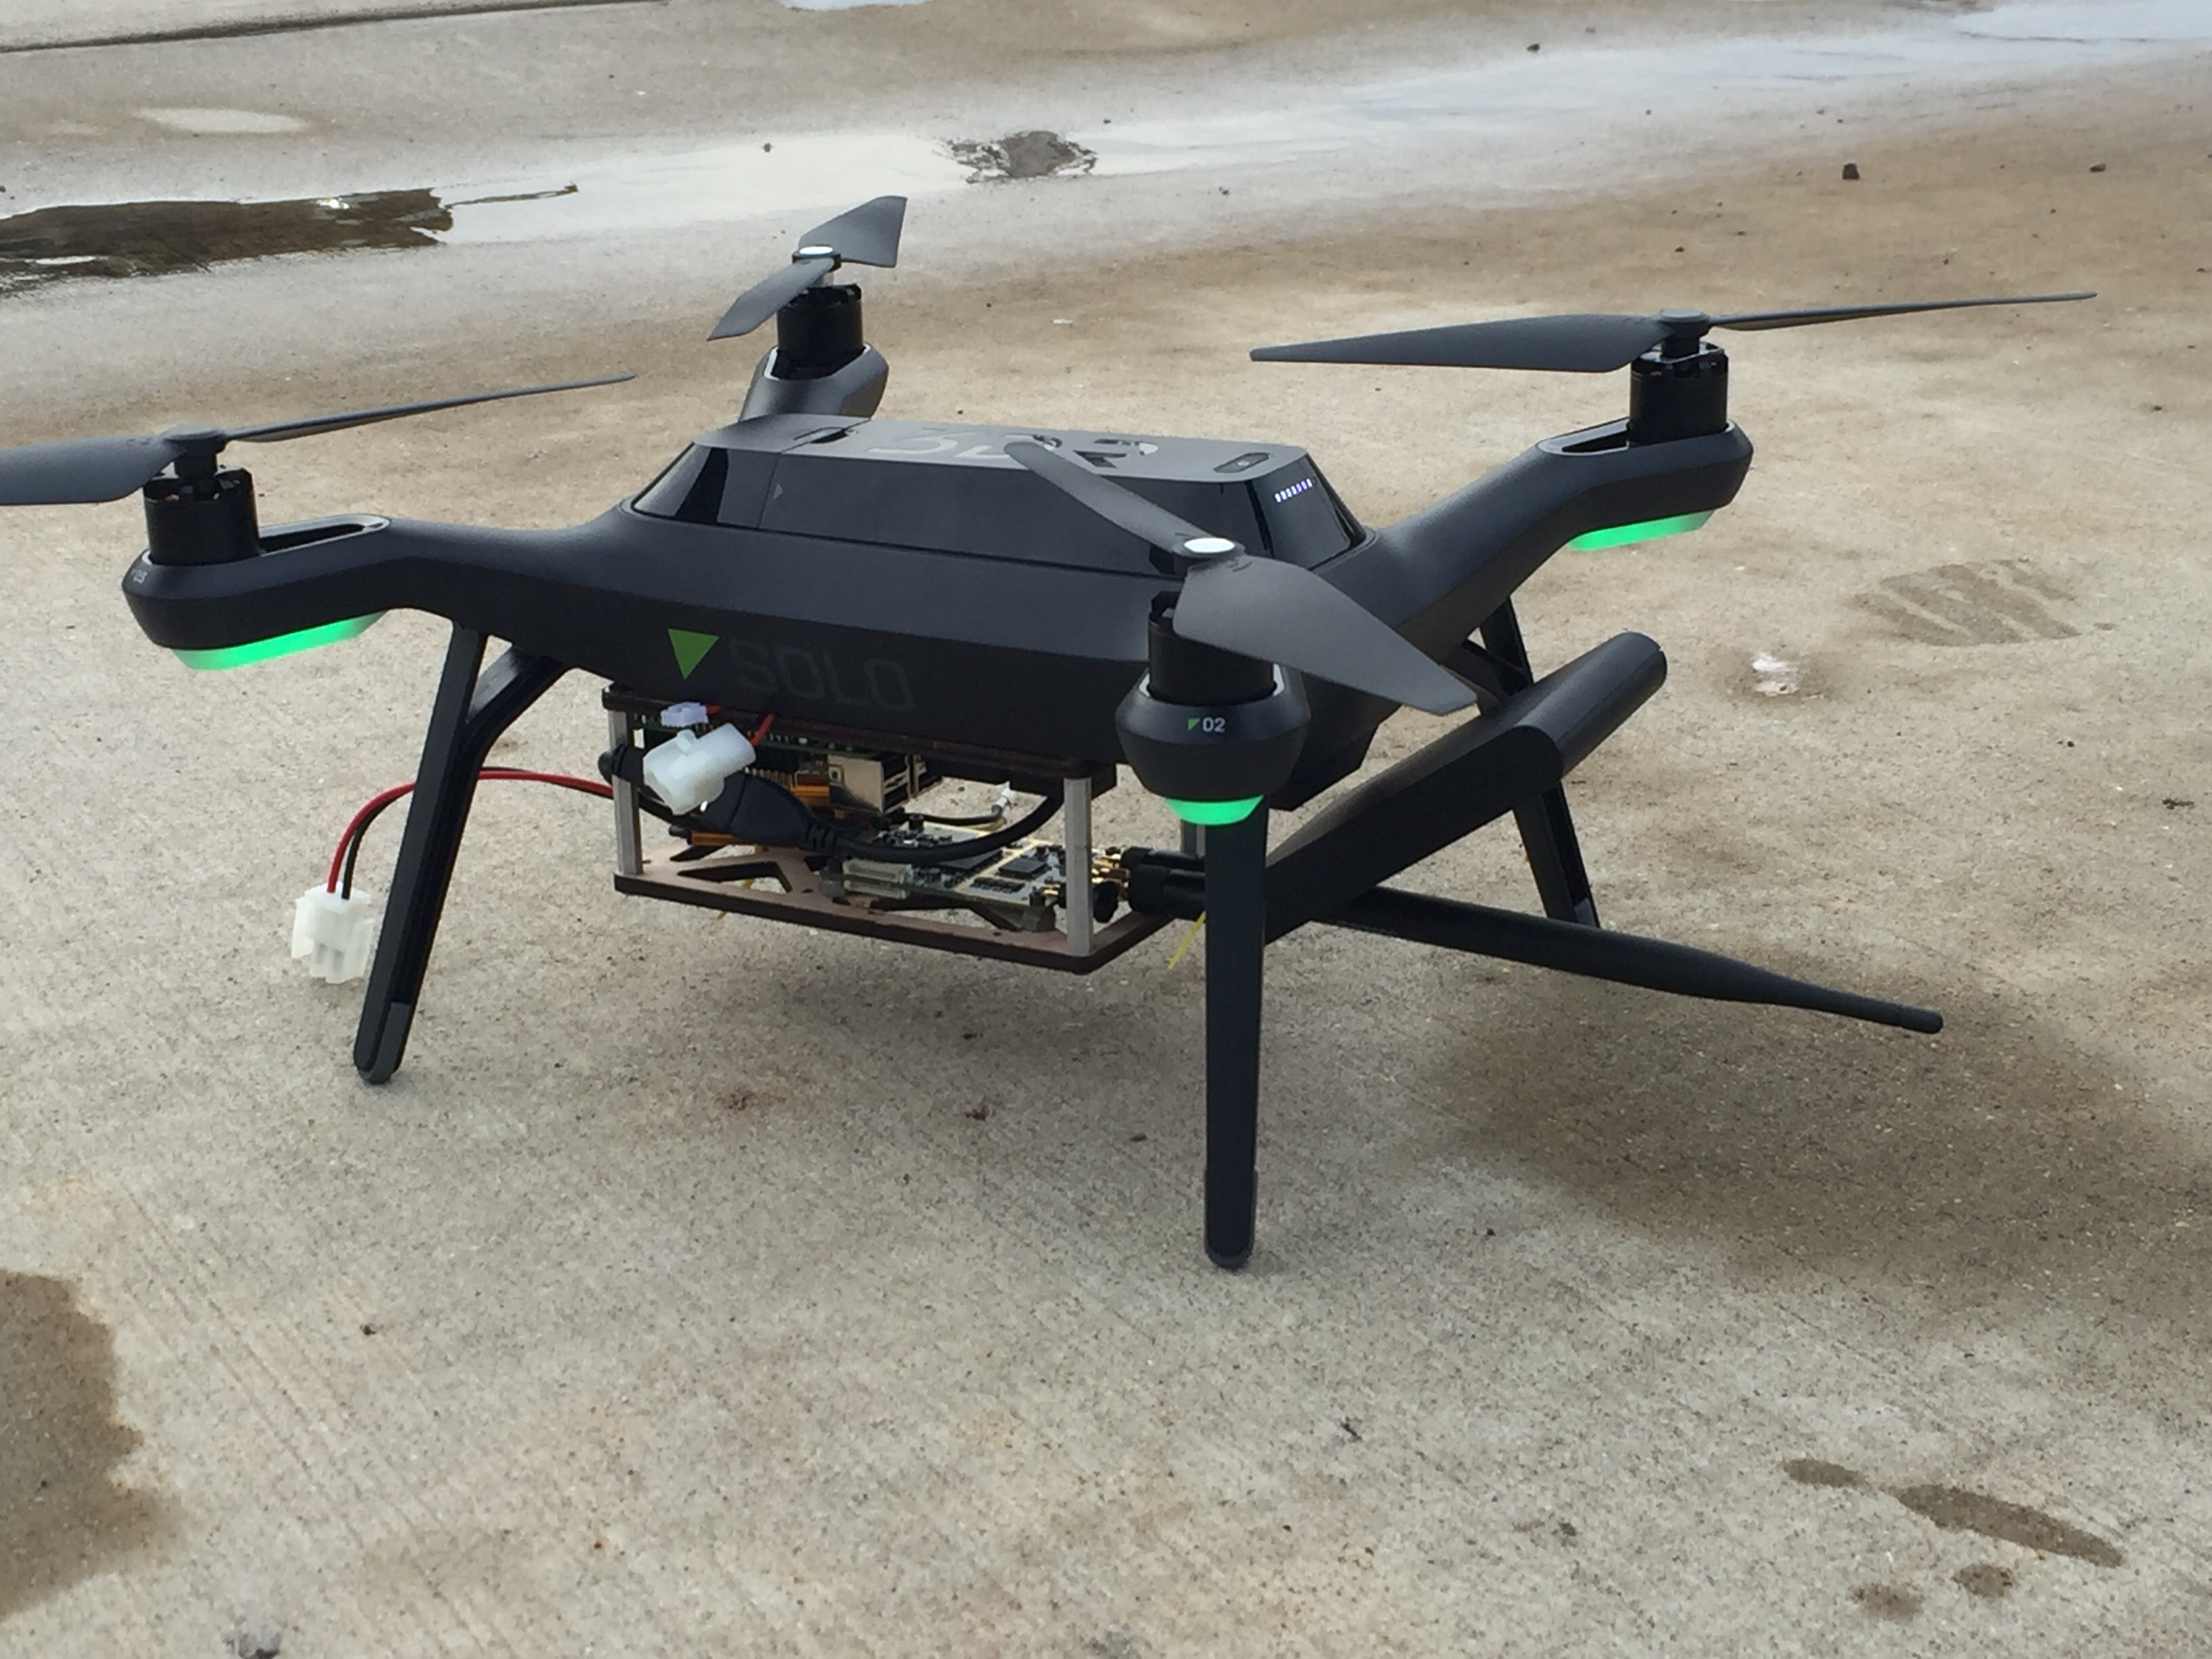
\includegraphics[width=0.45\textwidth]{img/drone_and_box.jpg}
  \caption{The complete system mounted on the drone. In flight testing was done with this setup.}
  \label{fig:drone_and_box}
\end{figure}

\par\subsection{Spectrum Sensing}

In order to monitor the signal strength of our received data, the RSSI localization technique was used. RSSI was measured by taking the average signal power across a 20 MHz 802.11 wifi channel. This measurement was taken by using the USRP B200 Mini’s get\_rx\_sensor command.  This command returns the corresponding RSSI value as a double in dBm format.  Since a WiFi transmitter is not transmitting all of the time, there are sharp changes in RSSI measurements, as the USRP is receiving both when there is a signal and when there is none.

\begin{figure}[h!]
  \centering
  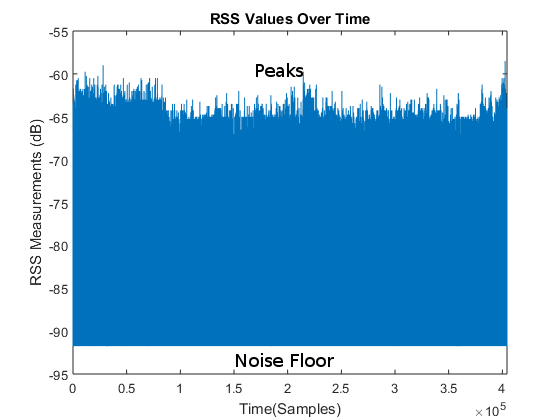
\includegraphics[width=0.45\textwidth]{img/rss_vals_test_labeled.png}
  \caption{This graph shows how the RSSI of our received signal can dramatically change.  These sharp transitions in RSSI values are due to the transmitter not always continually transmitting.}
  \label{fig:rss_values}
\end{figure}
In order to have an accurate measurement, RSSI reports that are under the noise floor must be filtered out. A detection threshold of -85 dBm was selected, as it is above the noise floor.  The output RSSI measurements only record noticeable signals.  

Corresponding RSSI values were used to estimate the distance of the transmission that was sensed.  The localization algorithm depended upon this calculation in order to accurately locate a signal source. the distance equation used was:

 \begin{align}
\label{eq:rss} RSSI &= 10\alpha log(d) \\ 
d &= 10^{(RSSI-RSSI_{calibration})(-10\alpha)} + d_{calibration} \label{eq:rss_dist}
\end{align}\\
These equations were mentioned previously in Section \ref{back:radio_loc}. 
Based on some field testing, this equation has been fairly accurate.\par

\begin{table}[ht]
\centering
\caption{The RSSI to distance calculation reasonably relates received signal strength to how far away a transmitter is located.}
\label{table:RSSI_Results}
\begin{tabular}{|l|l|l|} \hline
  RSSI (dBm) & Observed Distance (Meters) & Theoretical Distance (Meters) \\ \hline
  -50 & 3 & 3.2 \\
  -60 & 9 & 10 \\
  -70 & 26 & 31.62 \\ \hline
\end{tabular}
\end{table}\par

When the drone was tested, received signal strengths were between -65 to -80 dBm. These values fall within the expected power range of desired signals, as the sensing platform was 100 ft or 30 meters away from the transmitter. \par
%IQ_TO_FILE
In addition to calculating RSSI values, a C++ program separate from the code framework
was written. This program, called iq\_to\_file, was created as a foundation with 
which to work with. It became the testbed for specific elements of MASDR, since it
was already capable of logging. The code for this section is in Appendix \ref{app:iq_to_file}. 
This program is built on the rx\_samples\_to\_file example that Ettus Research provides 
with the UHD. This program already had the desired base functionality, so it proved
to be a good starting point. The program was then stripped of unnecessary functionality,
including the command-line interface. \par
With the extraneous functionality removed, components of the MASDR framework were
added, in order to test them separately. The matched filter, RSS measurements, 
and GPS modules were the sections added. This allowed for post-process localization. In order to 
save these values properly, they were packed into the complex type that was being
used to save IQ samples. In order to make it possible to pull these values out
in post-processing, they were given an unrealistic imaginary value. with each different 
module getting a different imaginary value. The matched filter outputs got 
a flag of 1000. GPS X, Y and Z coordinates were given flags of 2000, 3000, and 4000,
respectively. RSS values got a flag of 5000. These values were written with each 
buffer of samples received. This makes it easier to align results when processing.\par
%MATLAB
Once a data file was recorded, it was processed using a MATLAB script. This script 
is in Appendix \ref{app:matlab_proc}. This script reads in the .dat file produced 
by iq\_to\_file, as floats. It then separates the data into in-phase and quadrature
components. Then, after pre-allocating buffers, the script pulls out the non-IQ 
samples. The matched filter values and the RSS measurements are then plotted. The
script used to plot the received signal, but with longer record times, this
becomes impractical or impossible.
%Mapping Script
The script used to display the measured signal strengths was designed for post-proccesing use, taking in a text file of locations and their corresponding RSS values. The processing portion of the script is written in python, and can be found in Appendix \ref{app:mapping_script}. Equation (\ref{eq:rss_dist}) is used to calculate the raw distance to the signal. The Pythagorean Theorem is then used to eliminate the altitude component of the distance as can be seen in Figure \ref{fig:dist_pyth}. The latitude, longitude, and land-based distance are then formatted into a template string for each point at which a signal was detected.\par
\begin{figure}[h!]
\centering
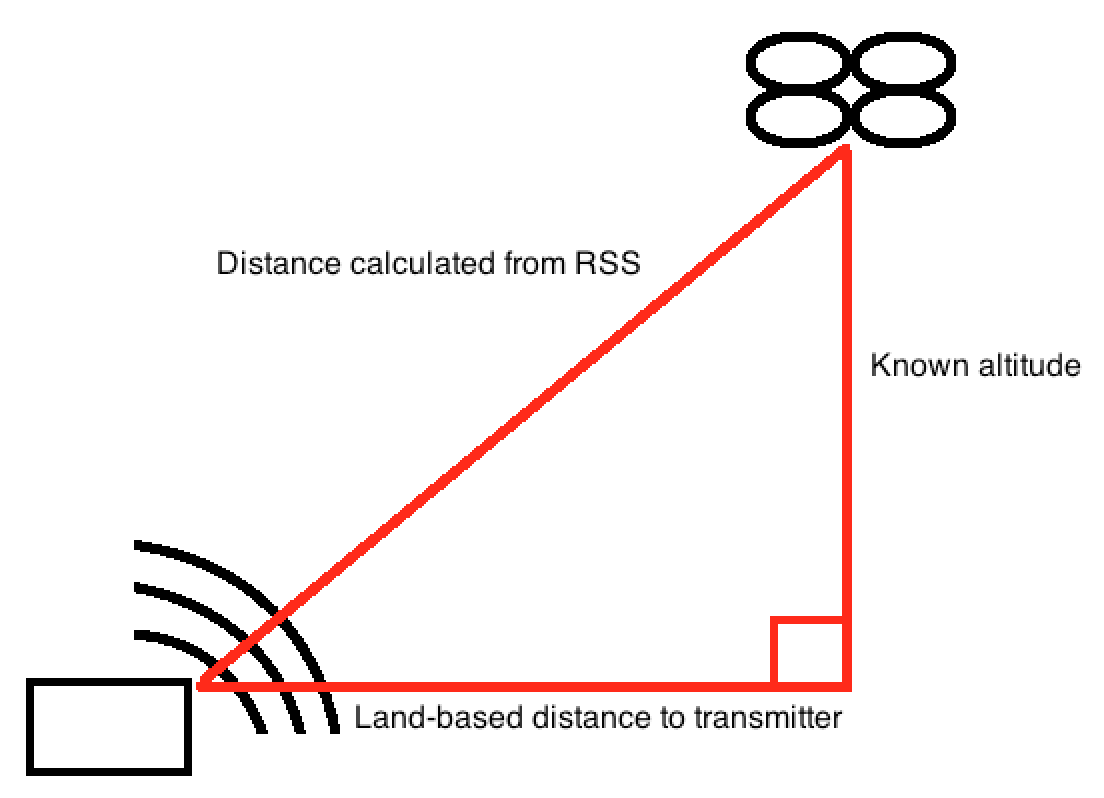
\includegraphics[width=0.45\textwidth]{img/distance_pythag_diagram.png}
\caption{Diagram showing right triangle used to calculate land-based distance from the calculated distance and a known altitude.}
\label{fig:dist_pyth}
\end{figure}
The formatted strings are inserted into a template html file, primarily composed of a Javascript block that calls into the Google Maps API. Using the drawing tools in the API, rings are drawn on the map corresponding to the calculated distance. An example output screenshot of a generated map has been included in Figure \ref{fig:map_localize}. The actual output is a webpage with a Google Maps instance running in it, so the map is fully interactive, with the ability to zoom in and scroll around as well.\par
\begin{figure}[h!]
\centering
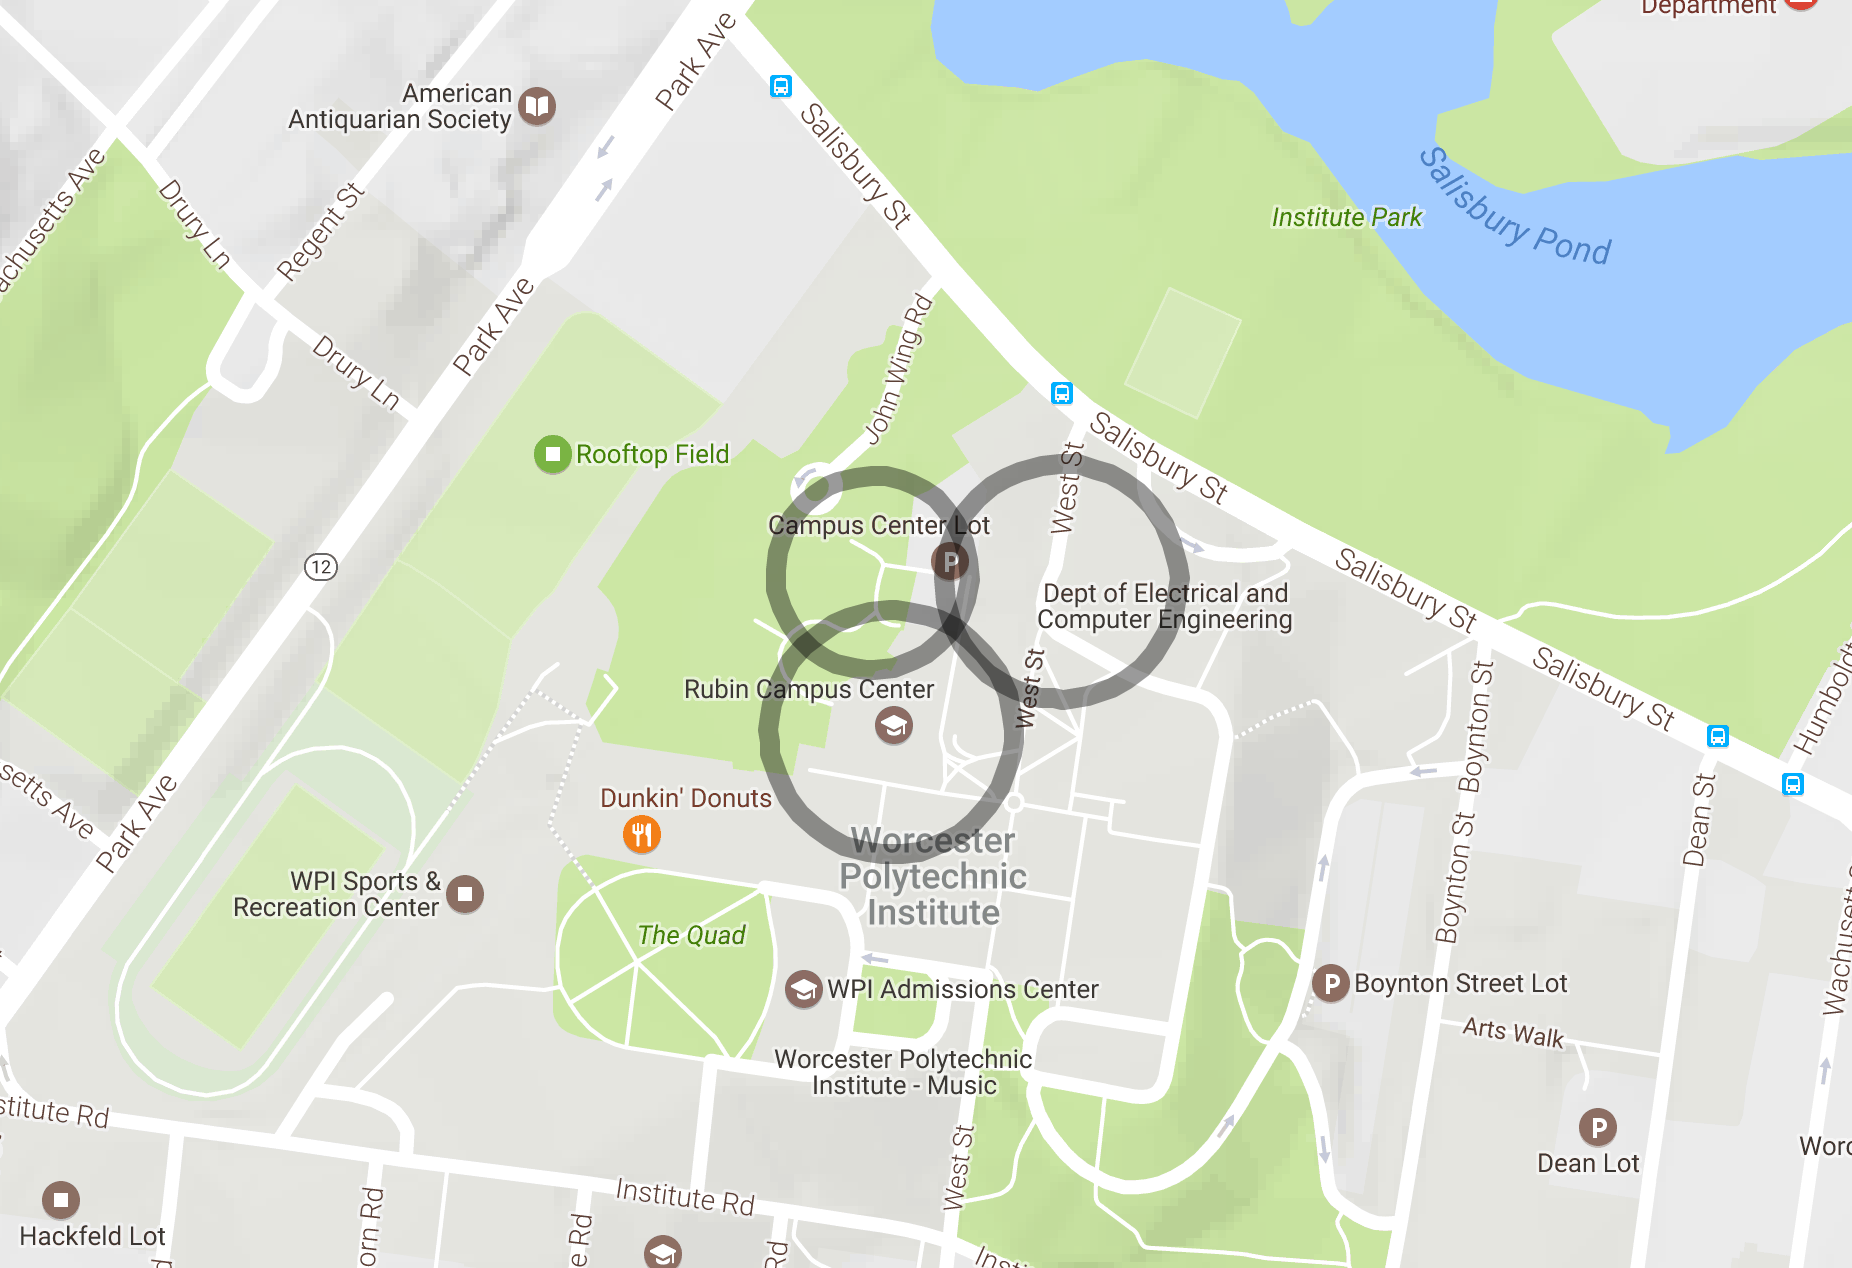
\includegraphics[width=0.45\textwidth]{img/localization_map_visualization.png}
\caption{Map-based localization example. The rings drawn are calculated from RSS values based on samples taken at the centers of each ring.}
\label{fig:map_localize}
\end{figure}
\section{Platform Deployment}
The platform on the 3DR Solo was tested in the two most applicable scenarios, the rural environment and the urban environment. The tests were conducted in secluded areas to prioritize privacy and safety concerns. The tests consisted of mounting the platform onto the 3DR Solo, flying the drone in a procedural flight path as seen in Figure \ref{fig:test_setup} to collect IQ data, and processing the data for the mapping and the localization of signals around that area. The signals in our case, would be the controller access point. 

\begin{figure}[ht!]
  \centering
  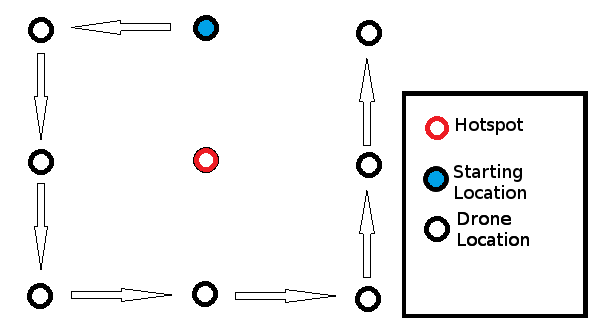
\includegraphics[width=0.45\textwidth]{img/Test_Plan_legend.png}
  \caption{3x3 diagram of test flight plan. The red circle represents where the controller was placed, and the blue circle represents where the drone was started.}
  \label{fig:test_setup}
\end{figure} \par

The simulation of the rural environment was organized at Professor Wyglinski's property on December 11th, 2016. In order to get the least interfering wifi signals, he turned off his WiFi, and he authorized the flight of the drone on his property. The testing environment consisted of high rise trees that surrounded the area and grew up to an average of 80ft. The resulting mapping and localization of the area is provided in Figure \ref{fig:rural_test}.

\begin{figure}[ht!]
  \centering
  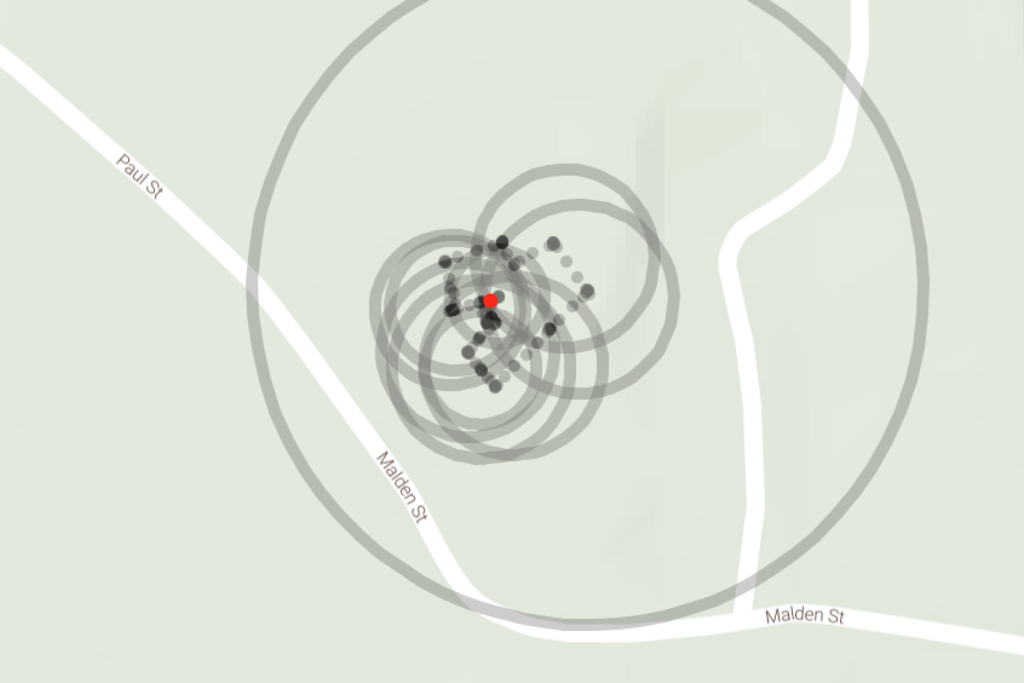
\includegraphics[width=0.45\textwidth]{img/ruraltest.png}
  \caption{The result of the test flight in a rural environment. The red dot shows where the actual access point was located. The black dots represent the GPS locations of where the drone traveled, and the their shades illustrate the length of time the drone was at that location. The black hollow circle depicts the localization of where the drone thinks the access point may be based on GPS and RSSI measurements. The larger hollow circle represents a measurement close to the noise floor.}
  \label{fig:rural_test}
\end{figure} \par
The simulation of the urban environment was organized at the Gateway Park garage on campus, on December 16th, 2016, after having gotten permission for the test from campus police. This WiFi of this area was uncontrolled, with various public and private access points active. This better simulated an urban environment. There were not many tall buildings around, limiting the applicability of the test on denser urban areas. As can be seen in Figure \ref{fig:urban_test}, the flight kept the platform relatively close to the controller, meaning that the strongest signal in the area would always be the controller. Even so, some of the points further from the controller read higher powers than would be expected from solely the controller, so it's likely that external Wi-Fi signals influenced the receptions, as was expected. This means that to effectively locate a transmitter in an urban environment, the platform must be closer to that transmitter than any other.
\begin{figure}[ht!]
    \centering
    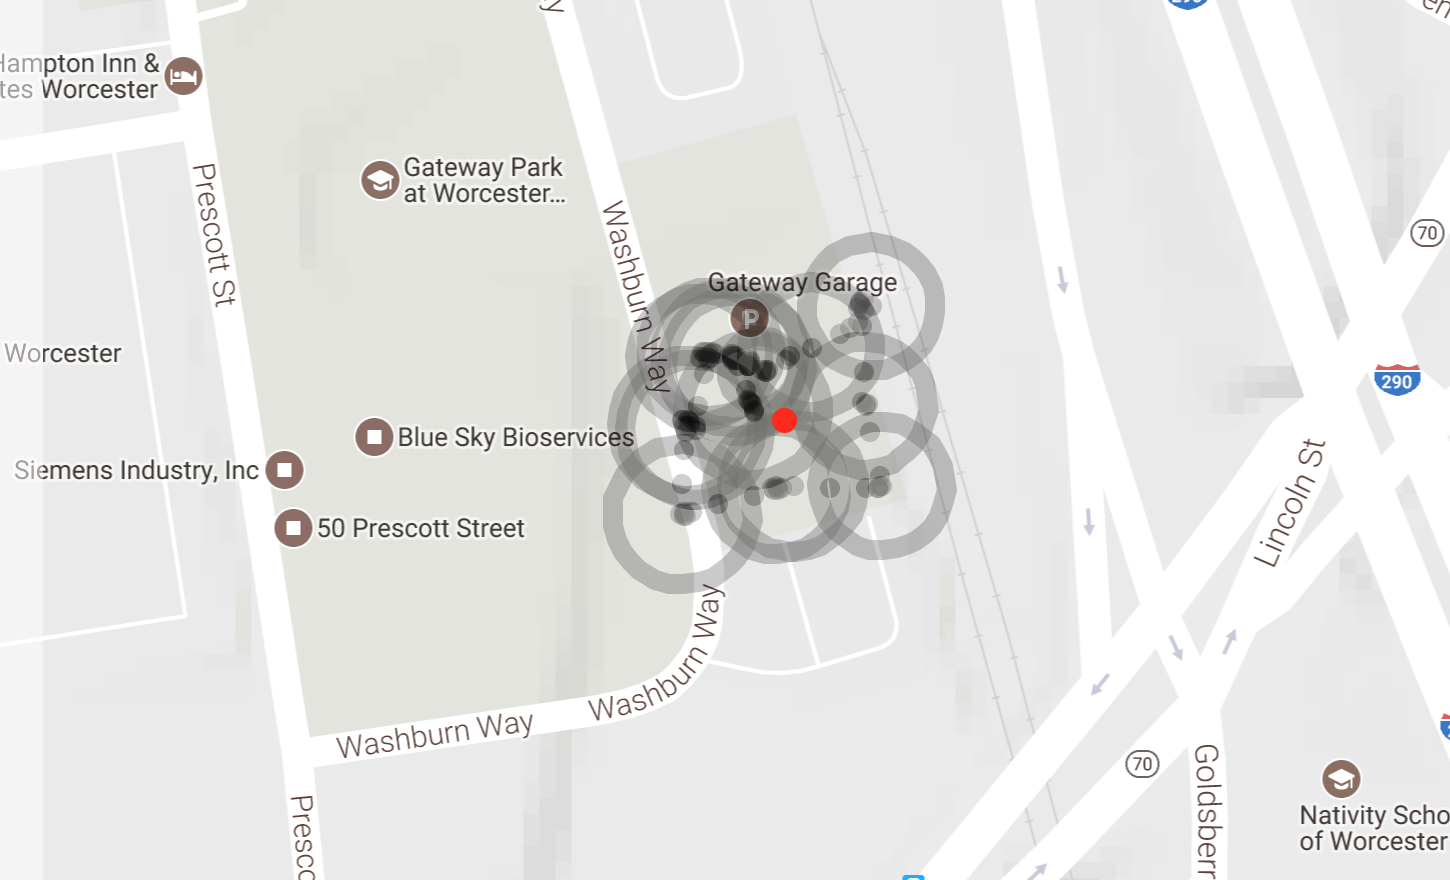
\includegraphics[width=0.45\textwidth]{img/urban_test_map.png}
    \caption{The result of the test flight in an urban environment. The red dot shows where the actual access point was located. The black dots represent the GPS locations of where the drone traveled, and the their shades illustrate the length of time the drone was at that location. The black hollow circle depicts the localization of where the drone thinks the access point may be based on GPS and RSSI measurements.}
    \label{fig:urban_test}
\end{figure} \par

\section{Conclusion}
In this paper we discussed multiple different technologies for UAS detection, their benefits and drawbacks.  We propose using spectrum sensing with radiolocation for the safe integration of UAS into the airspace. While there exists some limitations with the use of this technology, spectrum sensing is ideal in most scenarios, as the safe and successful operation of a UAV requires a wireless communication link.  There is a tradition of using wireless transmissions for surveillance of manned aircraft. Much of the same technology used for manned aircraft can be reused for unmanned aviation as well.

The discussion therein has focused on ground-based spectrum sensors. An opportunity exists to explore the possibility of airborne spectrum sensors for UAS DAA applications. 


% if have a single appendix:
%\appendix[Proof of the Zonklar Equations]
% or
%\appendix  % for no appendix heading
% do not use \section anymore after \appendix, only \section*
% is possibly needed

% use appendices with more than one appendix
% then use \section to start each appendix
% you must declare a \section before using any
% \subsection or using \label (\appendices by itself
% starts a section numbered zero.)
%


\appendices
\section{Proof of the First Zonklar Equation}
Appendix one text goes here.

% you can choose not to have a title for an appendix
% if you want by leaving the argument blank
\section{}
Appendix two text goes here.


% use section* for acknowledgment
\section*{Acknowledgment}


The authors would like to thank...


% Can use something like this to put references on a page
% by themselves when using endfloat and the captionsoff option.
\ifCLASSOPTIONcaptionsoff
  \newpage
\fi



% trigger a \newpage just before the given reference
% number - used to balance the columns on the last page
% adjust value as needed - may need to be readjusted if
% the document is modified later
%\IEEEtriggeratref{8}
% The "triggered" command can be changed if desired:
%\IEEEtriggercmd{\enlargethispage{-5in}}

% references section

% can use a bibliography generated by BibTeX as a .bbl file
% BibTeX documentation can be easily obtained at:
% http://mirror.ctan.org/biblio/bibtex/contrib/doc/
% The IEEEtran BibTeX style support page is at:
% http://www.michaelshell.org/tex/ieeetran/bibtex/
%\bibliographystyle{IEEEtran}
% argument is your BibTeX string definitions and bibliography database(s)
%\bibliography{IEEEabrv,../bib/paper}
%
% <OR> manually copy in the resultant .bbl file
% set second argument of \begin to the number of references
% (used to reserve space for the reference number labels box)
\begin{thebibliography}{1}

\bibitem{IEEEhowto:kopka}
H.~Kopka and P.~W. Daly, \emph{A Guide to \LaTeX}, 3rd~ed.\hskip 1em plus
  0.5em minus 0.4em\relax Harlow, England: Addison-Wesley, 1999.

\end{thebibliography}

% biography section
% 
% If you have an EPS/PDF photo (graphicx package needed) extra braces are
% needed around the contents of the optional argument to biography to prevent
% the LaTeX parser from getting confused when it sees the complicated
% \includegraphics command within an optional argument. (You could create
% your own custom macro containing the \includegraphics command to make things
% simpler here.)
%\begin{IEEEbiography}[{\includegraphics[width=1in,height=1.25in,clip,keepaspectratio]{mshell}}]{Michael Shell}
% or if you just want to reserve a space for a photo:

\begin{IEEEbiography}{Jonathan M. Peck}
earned a Bachelor of Science in Computer engineering in 2006 from Clarkson University and Master of Science in Electrical Engineering in 2012 from Syracuse University. He recently obtained a Masters of Business Administration from the State University of New York at Oswego. His past experience is in the design of electronic warfare systems applied to wireless communications with an emphasis on detector design, system modeling, and simulation. His research interest include UAS wireless communications and practical radiolocation systems. He is licensed remote pilot by the FAA under Part 107 for operation of UAS.
\end{IEEEbiography}

% if you will not have a photo at all:
\begin{IEEEbiographynophoto}{John Doe}
Biography text here.
\end{IEEEbiographynophoto}

% insert where needed to balance the two columns on the last page with
% biographies
%\newpage

\begin{IEEEbiographynophoto}{Jane Doe}
Biography text here.
\end{IEEEbiographynophoto}

% You can push biographies down or up by placing
% a \vfill before or after them. The appropriate
% use of \vfill depends on what kind of text is
% on the last page and whether or not the columns
% are being equalized.

%\vfill

% Can be used to pull up biographies so that the bottom of the last one
% is flush with the other column.
%\enlargethispage{-5in}



% that's all folks
\end{document}


